 \iffalse
\chapter{2007}
\author{EE24BTECH11021 - Eshan Ray}
\section{ae}
\fi
    \item Combustion between fuel \brak{octane} and oxidizer \brak{air} occurs inside a combustor with the following stoichiometric chemical reaction $\colon$
    $$2C_{8}H_{18}+\brak{25O_2+94N_2}\longrightarrow 16CO_2+18H_2O+94N_2$$
    The atomic weights of carbon \brak{C}, hydrogen \brak{H},oxygen \brak{O}, and nitrogen \brak{N} are $12,1,16,\, and\,14$, respectively. If the combustion takes place  with the fuel to air ratio $0.028$, then the equivalence ratio of the fuel-oxidizer mixture is
    \begin{enumerate}
        \item $0.094$
        \item $0.422$
        \item $0.721$
        \item $2.371$
    \end{enumerate}
    \item The von Mises yield criteria or the maximum distortion energy criterion for a plane stress problem with $\sigma_1$ and $\sigma_2$ as the principal stresses in the plane, and $\sigma_Y$ as the yield stress, requires
    \begin{enumerate}
        \item $\sigma_1^2-\sigma_1\sigma_2+\sigma_2^2\leq \sigma_Y^2$
        \item $\abs{\sigma_1-\sigma_2}\leq\sigma_Y$
        \item $\abs{\sigma_1}\leq \sigma_Y$
        \item $\abs{\sigma_2}\leq\sigma_Y$
    \end{enumerate}
    \item An Euler-Bernoulli beam having a rectangular cross-section, as shown in the figure, is subjected to a non-uniform bending moment along its length. $V_z=\frac{dM_y}{dx}$. The shear stress distribution $\tau_{xz}$ across its cross- section is given by 

   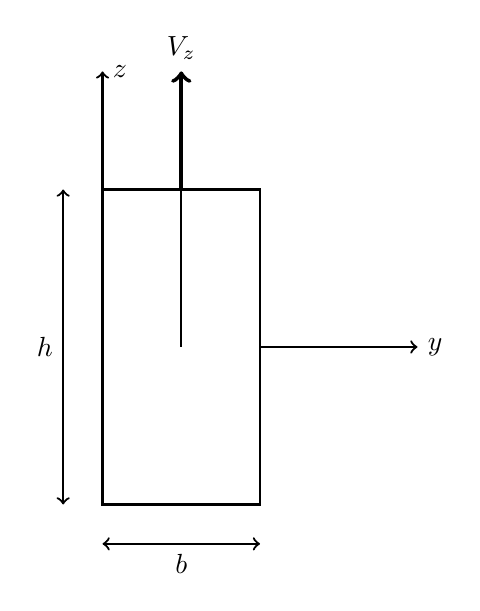
\begin{tikzpicture}
    % Draw the rectangle
    \draw[thick] (0,0) rectangle (2,4);
    
    % Draw the vertical line inside the rectangle
    \draw[thick] (1, 4) -- (1, 2);

    % Draw the vertical arrow (Vz) with ultra thickness
    \draw[->, ultra thick] (1, 4) -- (1, 5.5) node[anchor=south] {$V_z$};

    % Draw the horizontal arrow (y direction)
    \draw[->, thick] (2, 2) -- (4, 2) node[anchor=west] {$y$};

    % Label the width (b) and height (h)
    \draw[<->, thick] (0, -0.5) -- (2, -0.5) node[midway, anchor=north] {$b$};
    \draw[<->, thick] (-0.5, 0) -- (-0.5, 4) node[midway, anchor=east] {$h$};

    % Label the z-axis
    \draw[->, thick] (0, 0) -- (0, 5.5) node[anchor=west] {$z$};

\end{tikzpicture}
    \begin{enumerate}
        \item $\tau_{xz}=\frac{V_z}{2I_y}\frac{z}{\brak{\frac{h}{2}}}$
        \item $\tau_{xz}=\frac{V_z\brak{\frac{h}{2}}^2}{2I_y}\brak{1-\frac{z^2}{\brak{\frac{h}{2}}^2}}$
        \item $\tau_{xz}=\frac{V_z}{2I_y}\brak{\frac{z}{\brak{\frac{h}{2}}}}^2$
        \item $\tau{_xz}=\frac{V_z\brak{\frac{h}{2}}^2}{2I_y}$
    \end{enumerate}
    \item At a stationary point of a multi-variable function, which of the following is true?
    \begin{enumerate}
        \item Curl of the function becomes unity
        \item Gradient of the function vanishes
        \item Divergence of the function vanishes
        \item Gradient of the function is maximum
    \end{enumerate}
    \item In a rocket engine, the hot gas generated in the combustion chamber exits the nozzle with a mass flow rate $719\,\frac{kg}{sec}$ and velocity $1794\,\frac{m}{s}$. The area of the nozzle exit section is $0.635\,m^2$. If the nozzle expansion is optimum, then the thrust produced by the engine by
        \begin{enumerate}
            \item $811\, kN$
            \item $1290\, kN$
            \item $1354\, kN$
            \item $2172\, kN$
        \end{enumerate}
    \item For the control volume shown in the figure below, the velocities are measured both at the upstream and the downstream ends.

 \begin{circuitikz}
\tikzstyle{every node}=[font=\normalsize]
\draw (11.5,14.5) to[short] (11.5,11.5);
\draw (17.5,15.25) to[short] (17.5,10.75);
\draw [dashed] (11.5,14.5) -- (17.5,15.25);
\draw [dashed] (11.5,11.5) -- (17.5,10.75);
\draw [->, >=Stealth] (10.5,14.5) -- (11.5,14.5);
\draw [->, >=Stealth] (10.5,14.25) -- (11.5,14.25);
\draw [short] (10.5,14.5) -- (10.5,11.5);
\draw [->, >=Stealth] (10.5,14) -- (11.5,14);
\draw [->, >=Stealth] (10.5,13.75) -- (11.5,13.75);
\draw [->, >=Stealth] (10.5,13.5) -- (11.5,13.5);
\draw [->, >=Stealth] (10.5,13.25) -- (11.5,13.25);
\draw [->, >=Stealth] (10.5,13) -- (11.5,13);
\draw [->, >=Stealth] (10.5,12.75) -- (11.5,12.75);
\draw [->, >=Stealth] (10.5,12.5) -- (11.5,12.5);
\draw [->, >=Stealth] (10.5,12.25) -- (11.5,12.25);
\draw [->, >=Stealth] (10.5,12) -- (11.5,12);
\draw [->, >=Stealth] (10.5,11.75) -- (11.5,11.75);
\draw [->, >=Stealth] (10.5,11.5) -- (11.5,11.5);
\draw [->, >=Stealth] (17.5,15.25) -- (19,15.25);
\draw [short] (19,15.25) -- (17.5,13);
\draw [->, >=Stealth] (17.5,15) -- (18.82,15);
\draw [->, >=Stealth] (17.5,14.75) -- (18.65,14.75);
\draw [->, >=Stealth] (17.5,14.5) -- (18.49,14.5);
\draw [->, >=Stealth] (17.5,14.25) -- (18.32,14.25);
\draw [->, >=Stealth] (17.5,14) -- (18.18,14);
\draw [->, >=Stealth] (17.5,13.75) -- (18,13.75);
\draw [->, >=Stealth] (17.5,13.5) -- (17.82,13.5);
\draw [->, >=Stealth] (17.5,10.75) -- (19,10.75);
\draw [short] (17.5,13) -- (19,10.75);
\draw [->, >=Stealth] (17.5,11.25) -- (18.69,11.25);
\draw [->, >=Stealth] (17.5,11.75) -- (18.33,11.75);
\draw [->, >=Stealth] (17.5,12.25) -- (18,12.25);
\draw [->, >=Stealth] (17.5,11) -- (18.82,11);
\draw [->, >=Stealth] (17.5,11.5) -- (18.53,11.5);
\draw [->, >=Stealth] (17.5,12) -- (18.2,12);
\draw [->, >=Stealth] (17.5,12.5) -- (17.8,12.5);
\draw  (14.25,13.25) ellipse (1.5cm and 0.25cm);
\draw [<->, >=Stealth] (17.25,15.25) -- (17.25,13);
\draw [<->, >=Stealth] (17.25,13) -- (17.25,10.75);
\draw [short] (17.25,13) -- (16.5,13);
\draw [->, >=Stealth] (16.5,13) -- (16.5,13.75);
\node [font=\normalsize] at (11,15) {$U_{\infty}$};
\node [font=\normalsize] at (18,15.75) {$U_\infty$};
\node [font=\normalsize] at (18,10.5) {$U_\infty$};
\node [font=\normalsize] at (17,14.25) {h};
\node [font=\normalsize] at (17,12) {h};
\node [font=\normalsize] at (16.5,14) {y};
\node [font=\normalsize] at (13.75,15.25) {streamline};
\node [font=\normalsize] at (13.75,10.75) {streamline};
\node [font=\normalsize] at (19,14.25) {$u= \frac{U_\infty}{h}y$};
\node [font=\normalsize] at (18.75,12.25) {$u= -\frac{U_\infty}{h}y$};
\end{circuitikz}\\
The flow of density $\rho$ is incompressible, two dimensional and steady. The pressure is $p_\infty$ over the entire surface of the control volume. The drag on the airfoil is given by,
        \begin{enumerate}
            \item $\frac{\rho U_\infty^2h}{3}$
            \item $0$
            \item $\frac{\rho U_\infty^2h}{6}$
            \item $2\rho U_\infty^2h$
        \end{enumerate}
    \item A gas turbine engine operates with a constant area duct combustor with inlet and outlet stagnation temperatures $540\, K$ and $1104\, K$ respectively. Assume that the flow is one dimensional, incompressible and frictionless and that the heat addition is driving the flow inside the combustor. The pressure loss, factor \brak{stagnation\,pressure\,loss\,non-dimentionalized\,by\,the\,inlet\,dynamic\,pressure} of the combustor is 
            \begin{enumerate}
                \item $0$
                \item $0.489$
                \item $1.044$
                \item $2.044$
            \end{enumerate}
    \item The diffuser of an airplane engine decelerates the airflow from the flight Mach number $0.85$ to the compressor inlet Mach number $0.38$. Assume that the ratio of the specific heats is constant and is equal to $1.4$. If the diffuser pressure recovery ratio is $0.92$, then the isentropic efficiency of the diffuser is
        \begin{enumerate}
            \item $0.631$
            \item $0.814$
            \item $0.892$
            \item $1.343$
        \end{enumerate}
    \item An airfoil section is known to generate lift when placed in a uniform stream of speed $U_\infty$ at an incidence $\alpha$. A biplane consisting of two such sections of identical chord $c$, separated by a distance $h$, is shown in the following figure

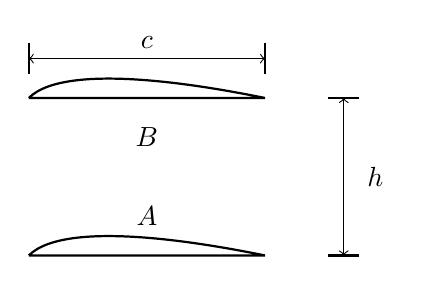
\begin{tikzpicture}

    % Draw the airfoil shape (simplified)
    \draw[thick] (0,0) .. controls (0.5,0.5) and (2.5,0.1) .. (3,0) -- (0,0);
    \begin{scope}[yshift=-2cm]
      \draw[thick] (0,0) .. controls (0.5,0.5) and (2.5,0.1) .. (3,0) -- (0,0);
     \end{scope}
    % Draw the chord line
    \draw[<->] (3,0.5) -- (0,0.5);
    \draw[thick] (3,0.7) -- (3,0.3);
    \draw[thick] (0,0.7) -- (0,0.3);
    \draw[<->] (4,0) -- (4,-2);
    \draw[thick] (3.8,0) -- (4.2,0);
    \draw[thick] (3.8,-2) -- (4.2,-2);
    % Add label c for chord length
    \node at (1.5,0.7) {$c$};
    
    % Add B below the airfoil
    \node at (1.5,-0.5) {$B$};
    \node at (1.5,-1.5) {$A$};
    \node at (4.4,-1) {$h$};
\end{tikzpicture}

With regard to this biplane, which of the following statements is true?
    \begin{enumerate}
        \item Both the airfoils experience an upwash and an increased approach velocity
        \item Both the airfoils experience an downwash and an decreased approach velocity
        \item Both the airfoils experience an upwash and airfoil $A$ experience a decreased approach velocity while airfoil $B$ experiences  an increased approach velocity
        \item The incidence for the individual sections of the biplane is not altered
    \end{enumerate}
    \item  Numerical value of the integral\\
    $J=\int_{0}^{1}\frac{1}{1+x^2}\, dx,$ if evaluated numerically using the Trapezoidal rule with $dx=0.2$ would be 
    \begin{enumerate}
        \item $1$
        \item $\frac{\pi}{4}$
        \item $0.7837$
        \item $0.2536$
    \end{enumerate}
    \item The purpose of  a fuel injection system in the combustor is
    \begin{enumerate}
        \item to accelerate the flow in the combustor
        \item to increase the stagnation pressure of the fuel-air mixture 
        \item to ignite the fuel-air mixture
        \item to convert the bulk fuel into tiny droplets
    \end{enumerate}
    \item Which of the following values is nearer to the vacuum specific impulse of a rocket engine using liquid engine hydrogen and liquid oxygen as propellants?
    \begin{enumerate}
        \item $49\,sec$
        \item $450\,sec$
        \item $6000\,sec$
        \item $40000\,sec$
    \end{enumerate}
    \item A circular cylinder is placed in an uniform steam of ideal fluid with its axis normal to the flow. Relative to the forward stagnation point, the angular positions along the circumference where the speed along the surface of the cylinder is equal to the free stream speed are 
    \begin{enumerate}
        \item $30,150,210\,and\,330\,degrees$
        \item $45,135,225\,and\,315\,degrees$
        \item $0,90,180\,and\,270\,degrees$
        \item $60,120,240\,and\,300\,degrees$
    \end{enumerate}
    \item The Newton-Raphson iteration formula to find a cube root of a positive number $c$ is
    \begin{enumerate}
        \item $x_{k+1}=\frac{2x_k^3+\sqrt[3]{c}}{3x_k^2}$
        \item $x_{k+1}=\frac{2x_k^3-\sqrt[3]{c}}{-3x_k^2}$
        \item $x_{k+1}=\frac{2x_k^3+c}{3x_k^2}$
        \item $x_{k+1}=\frac{x_k^3+c}{3x_k^2}$
    \end{enumerate}
    \item The torsion constant $J$ of a thin-walled closed tube of thickness $t$ and mean radius $r$ is given by
    \begin{enumerate}
        \item $J=2\pi rt^3$
        \item $J=2\pi r^3t$
        \item $J=2\pi r^2t^2$
        \item $J=2\pi r^4$
    \end{enumerate}
    \item An aerospace system shown in the following figure is designed in such a way that the expansion generated at $A$ is completely absorbed by  wall $B$ for $p_1=p_d$, where $p_d$ corresponds to the design condition.

   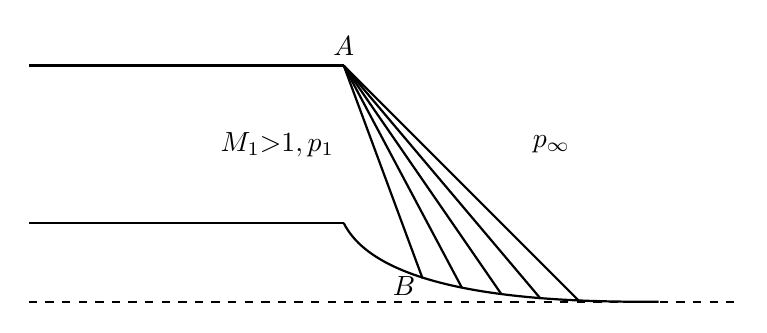
\begin{tikzpicture}

       \coordinate (O) at (0,0);
       \coordinate (A) at (4,0);
       \coordinate (C) at (0,-2);
       \coordinate (D) at (4,-2);

       \draw[thick] (4,-2) .. controls (4.5,-3) and (7,-3) .. (8,-3);
       \draw[thick] (0,0) -- (4,0);
       \draw[thick] (0,-2) -- (4,-2);
       \draw[thick, dashed] (0,-3) -- (9,-3);

    \draw[thick] (A) -- (5,-2.7);
    \draw[thick] (A) -- (5.5,-2.82);
    \draw[thick] (A) -- (6,-2.9);
    \draw[thick] (A) -- (6.5,-2.96);
    \draw[thick] (A) -- (7,-3);
       \node[above] at (A) {$A$};
       \node[right] at (4.5,-2.8) {$B$};
       \node[left] at (7,-1) {$p_\infty$};
       \node[left] at (4,-1) {$M_1\textgreater 1,p_1$};
    \end{tikzpicture}

    For $p_1\textgreater p_\infty$ which of the following statements is NOT true?
    \begin{enumerate}
        \item For $p_1\textless p_d$, the expansion fan from $A$ gets reflected from $B$ as a compression wave
        \item For $p_1\textgreater p_d$, the expansion fan from $A$ gets reflected from $B$ as an expansion wave
        \item For $p_1\textless p_d$, the expansion fan from $A$ gets reflected from $B$ as an expansion wave
        \item For $p_1\textgreater p_d$, $B$ always sees an expansion
    \end{enumerate}
    \item The span-wise lift distribution for three wings is shown in the following figure$\colon$
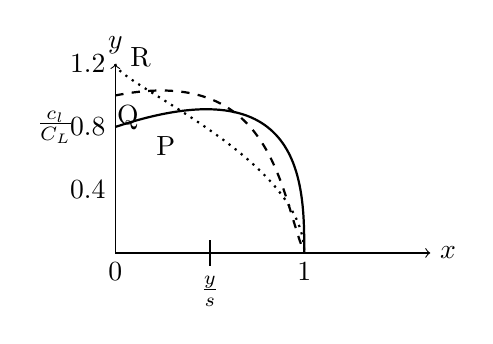
\begin{tikzpicture} [scale=0.8]

% Define the coordinate system
\coordinate (O) at (0,0);
\coordinate (X) at (5,0);
\coordinate (Y) at (0,3);

% Draw the axes
\draw[->] (O) -- (X) node[right] {$x$};
\draw[->] (O) -- (Y) node[above] {$y$};
\draw[thick] (1.5,0.2) -- (1.5,-0.2) node[below] {$\frac{y}{s}$};
% Add labels to the axes
\node[below] at (3,0) {1};
\node[left] at (0,3) {1.2};
\node[left] at (0,2) {0.8};
\node[left] at (0,1) {0.4};
\node[below] at (O) {0};
\node[left] at (-0.5,2) {$\frac{c_l}{C_L}$};
% Draw the curves
\draw[thick] (0,2) .. controls (3,3) and (3,1.1) .. (3,0); % Curve P
\draw[thick, dashed] (0,2.5) .. controls (2.5,3) and (2.6,1) .. (3,0); % Curve Q
\draw[thick, dotted] (0,3) .. controls (0,2.7) and (3,1.5) .. (3,0); % Curve R

% Add labels to the curves
\node[below] at (0.8,2) {P};
\node[below] at (0.2,2.5) {Q};
\node[above] at (0.4,2.8) {R};

\end{tikzpicture}

In the above figure, $c_l$ refers to the section lift coefficient, $C_L$ refers to the lift coefficient of the wing, $y$ is the coordinate along the span and $s$ is the span of the wing. A designer prefers to use a wing for which the stall begins at the root. Which of the wings will he choose?
    \begin{enumerate}
        \item $P$
        \item $Q$
        \item $R$
        \item None
    \end{enumerate}
